\chapter{Grundlagen}
\label{cha:grundlagen}
Zum Verstehen der Diskussion der Probleme der Blockchain-Technologie ist es notwendig, die grundlegenden Konzepte dieser zu verstehen. Weiterhin müssen allgemeine Anforderungen an \acs{B2B}-Anwendungen erfasst werden, anhand welchen die Diskussion erfolgt.

\section{Blockchain}

\subsection{Funktionsweise}
Die Funktionsweise der Blockchain wird in dieser Arbeit hauptsächlich am Beispiel von Bitcoin erklärt. Als erste Blockchain-Anwendung \cite{ZhengBlockchainChallengesOpportunities2017} und aufgrund der überschaubaren Komplexität liefert es die Grundlage für die Funktionsweise der Technologie. Andere Implementationen, wie Ethereum oder Ripple, funktionieren nach dem gleichen Prinzip.

\subsubsection{Allgemein}
Wenn der Begriff ``Die Blockchain'' auftaucht, ist damit meistens die Blockchain-Technologie gemeint. Es gibt nicht nur eine global bestehende Blockchain und auch nicht nur eine Implementation der Technologie, was beispielsweise anhand von Bitcoin und Ethereum ersichtlich ist.

Allgemein kann die Blockchain als Datenstruktur bezeichnet werden, welche verteilt, nicht lösch- und manipulierbar gespeichert werden kann. Weiterhin verifizieren jegliche Teilnehmer am Netzwerk ausgeführte Transaktionen, wodurch ein gemeinsamer Konsens über den Datenbestand besteht \cite{CrosbyBlockChainTechnologyBitcoin2016}.

In einer Blockchain werden Transaktionen in Blöcken gespeichert. Dabei handelt es sich um Operationen, welche Daten erstellen und manipulieren. Aus diesen lässt sich letztendlich der aktuelle Datenbestand ermitteln. So erfolgt beispielsweise bei Bitcoin keine Speicherung des aktuellen Guthabens der Teilnehmer. Es wird nur aus allen bestehenden Transaktionen berechnet \cite[S.~85]{AntonopoulosMasteringbitcoin2015}. Die letztendlich bestehenden Daten können beispielsweise Geldtransferinformationen (Bitcoin), Smart Contracts (Ethereum, selbst ausführende Verträge mit selbst erstellter Programmlogik, siehe \ref{subsec:use-cases}), simple Dokumente oder Informationen sein \cite{EthereumTeamEthereumWhitePaper2017}\cite{NakamotoBitcoinPeertoPeerElectronic2008}\cite{HyperledgerFabricTeamHyperledgerWhitepaper2016}. Die Blöcke setzen sich aus den Transaktionen sowie dem Block Header zusammen, welcher verschiedene Metadaten, wie zum Beispiel den kombinierten Hash\footnote{Hash: Ergebnis einer Operation, welche Daten in eine Zeichenfolge fester Länge umwandelt \cite[S.~\Rn{7}]{SwanBlockchainblueprintnew2015}.} aller Transaktionen, enthält \cite[S.~160-161]{AntonopoulosMasteringbitcoin2015}.

Die Blöcke sind miteinander verkettet. Jeder Block Header enthält den Hash  des vorherigen Block Headers (siehe Abb. \ref{fig:block-chain}). Dies ist ein wichtiges Feature zum Schutz der Blockchain vor Angriffen. Wenn ein Angreifer die Transaktionen eines Blocks zu seinen Gunsten verändert, würde sich der Hash des Block Headers ändern. Dieser müsste dann im darauffolgenden Block Header stehen, wodurch sich allerdings auch der Hash dieses Blocks ändert. Letztendlich müssten alle nachfolgenden Blöcke manipuliert werden, um eine gültige Blockchain zu erhalten \cite{NakamotoBitcoinPeertoPeerElectronic2008}. Diese Manipulation wird durch verschiedene Verfahren erschwert, welche genauer in den Kapiteln \ref{subsec:konsens} und \ref{subsec:immutability} erklärt werden.

\begin{figure}[!htbp]
  \centering
	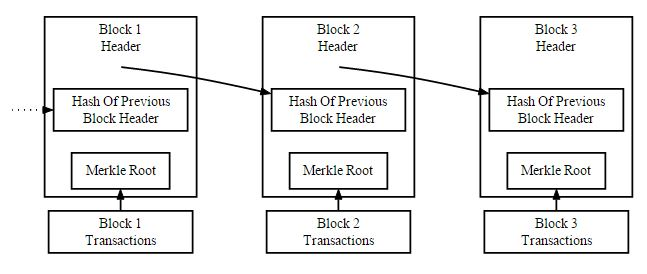
\includegraphics[width=0.87\textwidth,angle=0]{images/block-chain}
 	\caption{Verkettung von Blöcken durch Block Header Hashes \cite{RosicWhatHashingHood2017}.}
	\label{fig:block-chain}
\end{figure}

Die Blockchain ist verteilt gespeichert. Jeder Teilnehmer hat die Möglichkeit Sie auf seinem Rechner zu speichern. Somit besteht keine zentrale Instanz, welche die Kontrolle über die Daten hat. Weiterhin gibt es keinen Single Point of Failure\footnote{Single Point of Failure: Komponente eines Systems, dessen Ausfall den Ausfall des gesamten Systems bewirkt \cite{KshetriCanBlockchainStrengthen2017}.} \cite{KshetriCanBlockchainStrengthen2017}.

\label{subsec:konsens}
\subsubsection{Konsensmechanismen}
Aufgrund der verteilten Datenhaltung muss es Verfahren geben, um die Daten synchron und auf einem Stand, auf welchen sich alle Teilnehmer geeinigt haben, zu halten. Dazu gibt es die sogenannten Konsensmechanismen, welche gleichzeitig die Manipulierbarkeit der Daten verhindern. Bevor diese erklärt werden können, muss zunächst genauer auf die Funktion des Netzwerks eingegangen werden.

\paragraph{Funktion des Netzwerks}
Wenn ein Teilnehmer eine valide Transaktion (genauer im nächsten Absatz erklärt) ausführt, wird diese an alle Nodes\footnote{Node: Teilnehmer eines Blockchain-Netzwerks, welche die Blockchain speichern. Auch Peers genannt.} im Netzwerk weitergeleitet und im Transaktionspool aufgenommen. Dieser enthält alle noch nicht in Blöcken vorkommenden Transaktionen. Die Transaktionen werden von jeder Node in einen neuen Block aufgenommen. Gleichzeitig probiert jede Node den neuen Block zu erstellen. Dies wird durch verschiedene Konsensmechanismen realisiert. Bei Bitcoin und Ethereum findet der \acl{PoW} (\acs{PoW}) Anwendung (siehe unten). Sobald eine Node einen Block erstellt, wird dieser im Netzwerk verteilt. Jede Node hängt ihn an ihre lokale Blockchain an und beginnt mit der Erstellung des nächsten Blocks \cite[S.~200 ff.]{AntonopoulosMasteringbitcoin2015}.

Damit eine Transaktion valide ist, muss sie bestimmte Voraussetzungen erfüllen. So muss sie unter anderem mit dem Private Key des Senders signiert sein. Mittels seines Public Keys kann überprüft werden, ob wirklich er der Sender der Nachricht ist und ob die Transaktion manipuliert wurde. Dieses Verfahren wird auch in der Abbildung \ref{fig:key-signing} visualisiert. Durch das Signieren wird sichergestellt, dass ein Angreifer keine Transaktionen eines Nutzers manipulieren oder in seinem Namen ausführen kann. In Bitcoin ist eine weitere Kondition, dass der Transaktionsersteller die zu sendenden Bitcoins besitzen muss \cite[S.~18]{AntonopoulosMasteringbitcoin2015}. In Systemen wie Ethereum und Hyperledger Fabric, in welchen eigene Programmlogik abgebildet werden kann, können weitere Konditionen festgelegt werden. So muss beispielsweise ein Teilnehmer die nötigen Rechte haben, um eine Transaktion auszuführen \cite{HyperledgerComposerTeamAccessControlLanguage}.

\begin{figure}[!htbp]
	\centering
	  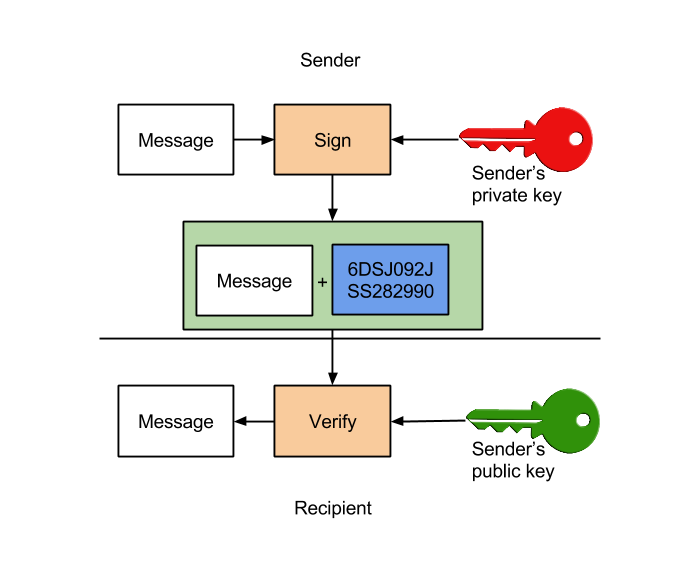
\includegraphics[width=0.35\textwidth,angle=0]{images/key-signing}
	  \caption{Signieren und Verifizieren von Nachrichten. Der Sender signiert die Nachricht mit seinem Private Key und der Empfänger kann diese mit den Public Key des Senders verifizieren \cite{WikimediaCommonsPublickeysigning2006}.}
	  \label{fig:key-signing}
\end{figure}
	
\paragraph{Proof-of-Work}
Der \acs{PoW} ist nur einer der zur Verfügung stehenden Konsensmechanismen (siehe Kapitel \ref{sec:eval-konsens}). Er bedarf jedoch genauerer Erklärung, da er in aktuellen Blockchain-Implementationen vorwiegend genutzt wird. Der \acs{PoW} ist eine Art Rätsel, welches mit der Rechenleistung von Nodes gelöst werden muss, um einen Block zu erschaffen (das sogenannte Mining). Genauer gesagt, muss für einen Block ein Hash gefunden werden, welcher einen bestimmten Wert unterschreitet. Um unterschiedliche Hashwerte für gleichbleibende Blöcke zu erhalten, gibt es im Block Header eine Nonce\footnote{Nonce: Eine Nummer, welche genau einmal für einen bestimmten Zweck genutzt wird \cite{MargaretNonceDefinition}.}, welche verändert wird \cite{NakamotoBitcoinPeertoPeerElectronic2008}. Alle Nodes im Netzwerk ändern diese so lange, bis ein gültiger Hash gefunden wird. Je kleiner der zu findende Hash ist, desto höher ist die Schwierigkeit. Aus Sicherheitsgründen ist es notwendig, dass die Blockerstellung eine gewisse Zeit benötigt. Um wachsender Rechenleistung und Teilnehmerzahl entgegenzuwirken und somit diese Zeit zu garantieren, kann die Schwierigkeit angepasst werden. Dies wird genauer im Kapitel \ref{sec:scalability-eval} erläutert. Damit die Nodes eine Motivation haben, Rechenleistung für das Erstellen von Blöcken zu nutzen, erhalten sie bei Erbringung des \acs{PoW} eine Belohnung sowie die Transaktionsgebühren in Form von Kryptowährung. In Verbindung mit den Mining sind auch Mining Pools zu erwähnen. Dabei handelt es sich um einen Zusammenschluss von Minern, welche gemeinsam probieren den \acs{PoW} zu erbringen. Gelingt dies, wird die Belohnung zwischen allen Teilnehmern im Pool geteilt.  \cite{NakamotoBitcoinPeertoPeerElectronic2008} \cite{EthereumTeamEthereumWhitePaper2017}. 

\paragraph{Forking}
Um vollständig zu verstehen, wie der \acs{PoW} funktioniert, muss das Forking erklärt werden. Wenn eine Node einen \acs{PoW} erbringt, also einen Block erstellt, wird dieser an alle anderen Nodes weitergeleitet. Im Bitcoin-Netzwerk dauert es bei einer maximalen Blockgröße von 1 MB \cite{SchererPerformanceScalabilityBlockchain2017}, zwischen 6 und 20 Sekunden, bis ein Block mindestens 90 \% aller Nodes erreicht hat \cite{BitcoinStatsBitcoinPropagationData}. Dies stimmt auch mit dem Paper von Decker und Wattenhofer überein, wo eine durchschnittliche Zeit von 12,6 Sekunden angegeben wird, bis ein Block 95 \% aller Nodes erreicht \cite{DeckerInformationpropagationbitcoin2013}. In dieser Zeit kann es vorkommen, dass eine weitere Node einen Block erstellt. Auch dieser wird im Netzwerk verteilt, wodurch zwei Versionen der Blockchain existieren: Eine endet mit Block A und die andere mit Block B. Dies ist der sogenannte Fork. Das Netzwerk muss sich nun darauf einigen, welche der beiden Versionen beibehalten werden soll. Deshalb gilt: Die Blockchain, in welche mehr Arbeit eingeflossen ist, ist die gültige. Im Falle von Bitcoin wäre dies die längere Blockchain. Die Nodes probieren an den zuerst erhaltenen Block (A oder B) einen neuen anzuhängen. Gelingt dies, ist eine der beiden Blockchains länger als die andere. Diese wird dann von allen Nodes als die richtige akzeptiert. Dieser Vorgang wird auch in den Abbildungen \ref{fig:fork_1} bis \ref{fig:fork_4} dargestellt. Theoretisch ist es möglich, dass ein Fork über mehrere Blöcke besteht. Die Wahrscheinlichkeit dafür ist jedoch gering, da mehrmals nacheinander mindestens zwei Nodes zur ungefähr gleichen Zeit einen Block erstellen müssen. Auch zu erwähnen ist, dass in einem Fork-Branch weitere Forks entstehen können. Diese Forks sind der Grund, warum Transaktionen erst als bestätigt gelten, sobald sie in einem Block stehen, welcher eine gewisse Anzahl an Nachfolgern hat. Denn erst dann ist die Sicherheit gegeben, dass die Transaktion nicht in einem Branch vorhanden ist, welcher eventuell verworfen wird \cite[S.~211 ff.]{AntonopoulosMasteringbitcoin2015}. Wie genau der \acs{PoW} das Netzwerk absichert, wird im Kapitel \ref{subsec:immutability} erklärt.

\begin{figure}[!htbp]
  \centering
    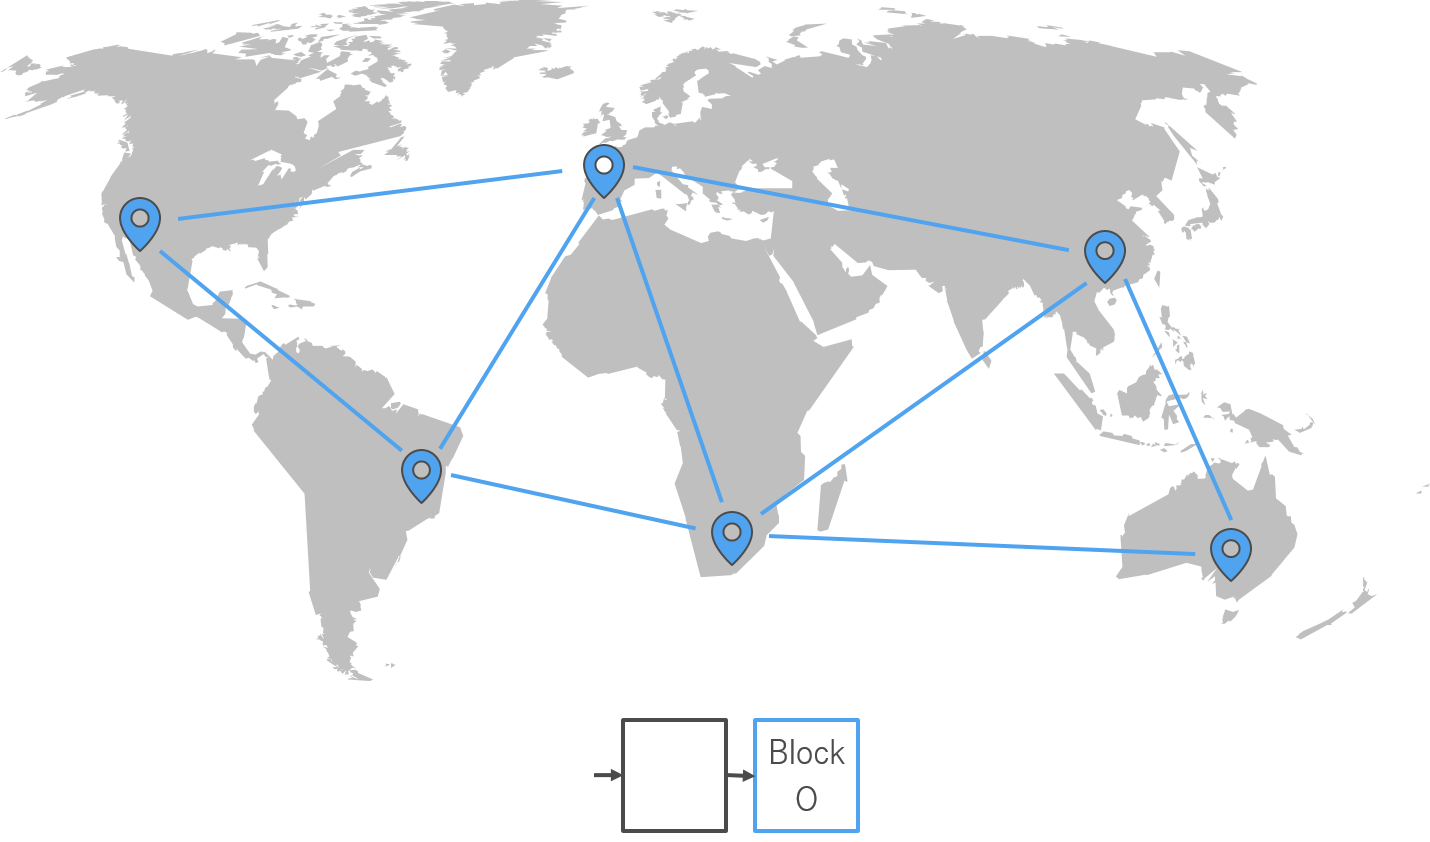
\includegraphics[width=0.85\textwidth,angle=0]{images/fork_1}
 	\caption{Fork-Visualisierung - Vor dem Fork besitzen alle Nodes Block O als letzten Block \cite[S.~200 ff.]{AntonopoulosMasteringbitcoin2015}.}
	\label{fig:fork_1}
\end{figure}

\begin{figure}[!htbp]
  \centering
	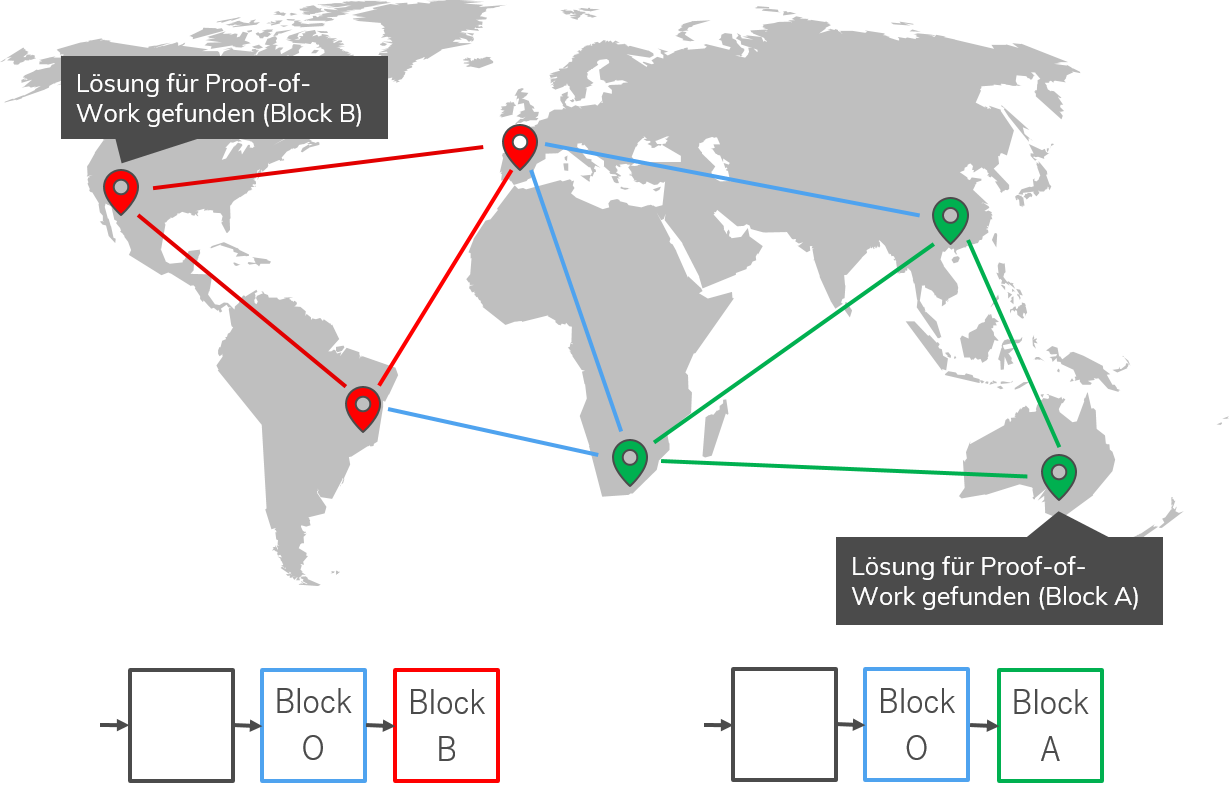
\includegraphics[width=0.85\textwidth,angle=0]{images/fork_2}
 	\caption{Fork-Visualisierung - zwei Nodes finden zur ungefähr gleichen Zeit einen Block und verbreiten ihn im Netzwerk, wodurch zwei Versionen der Blockchain bestehen \cite[S.~200 ff.]{AntonopoulosMasteringbitcoin2015}.}
	\label{fig:fork_2}
\end{figure}

\begin{figure}[!htbp]
  \centering
	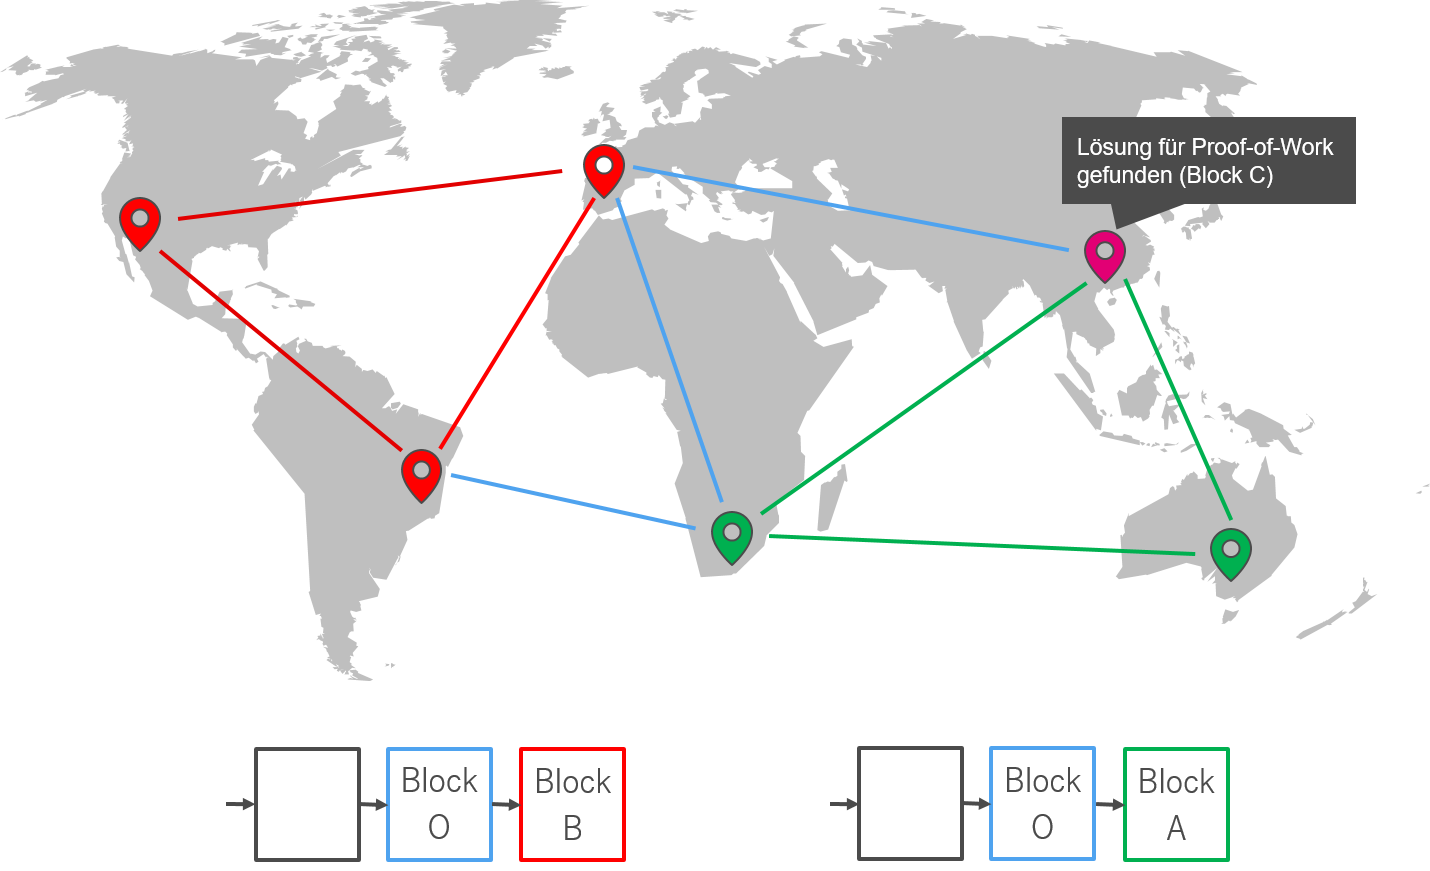
\includegraphics[width=0.85\textwidth,angle=0]{images/fork_3}
 	\caption{Fork-Visualisierung - Eine Node, welche Block A zuerst erhalten hat, hängt daran einen neuen Block C an \cite[S.~200 ff.]{AntonopoulosMasteringbitcoin2015}.}
	\label{fig:fork_3}
\end{figure}

\begin{figure}[!htbp]
  \centering
	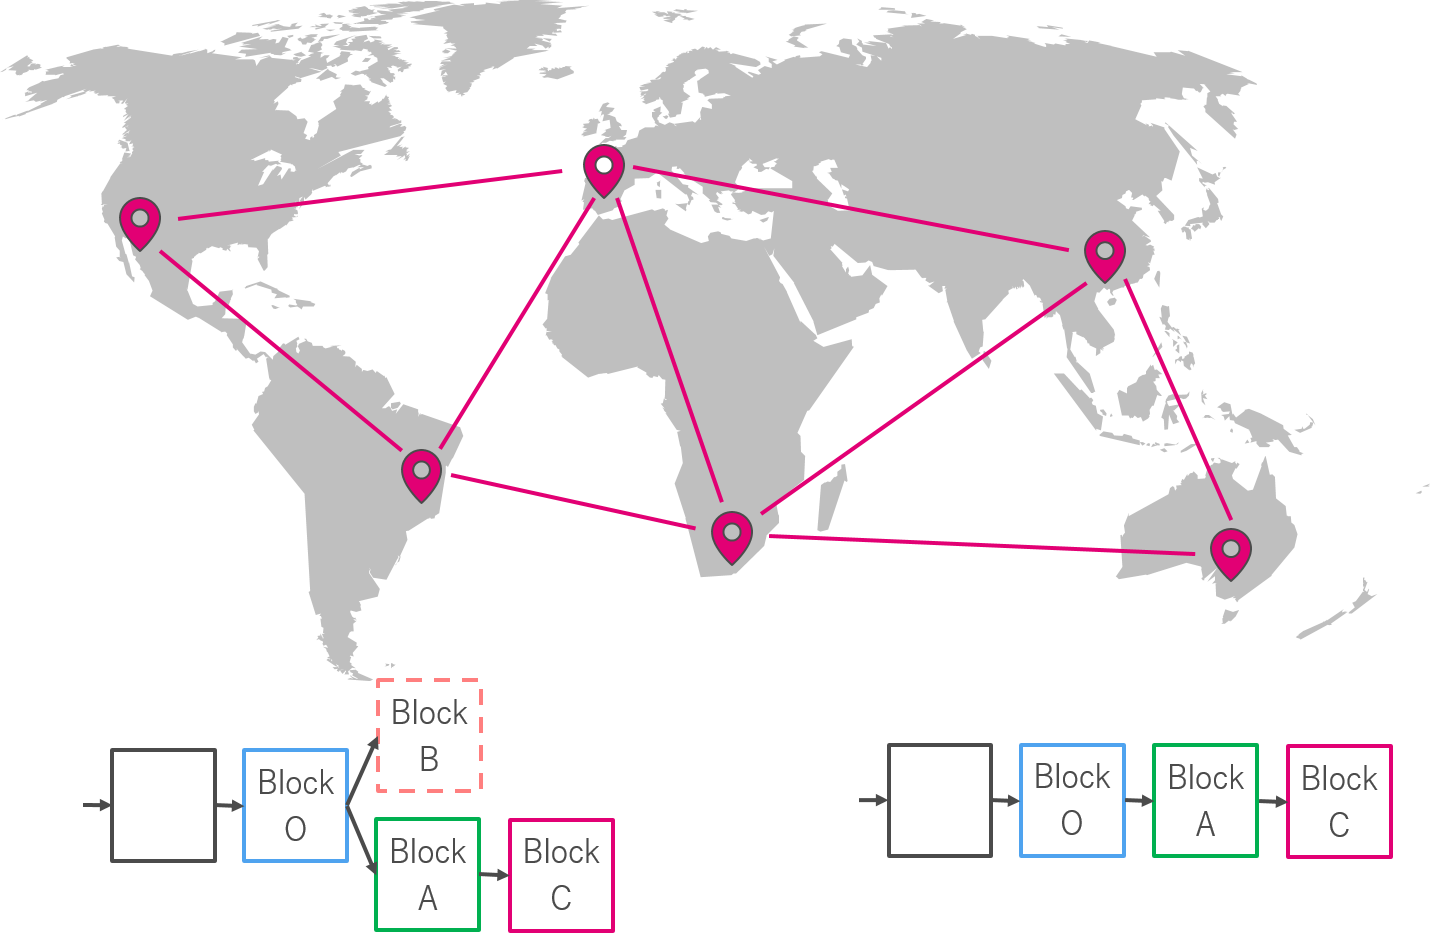
\includegraphics[width=0.85\textwidth,angle=0]{images/fork_4}
 	\caption{Fork-Visualisierung - Block C verbreitet sich im Netzwerk, rote Nodes sehen zwei Blockchains und akzeptieren die längere \cite[S.~200 ff.]{AntonopoulosMasteringbitcoin2015}.}
	\label{fig:fork_4}
\end{figure}

Neben dem \acs{PoW} gibt es noch weitere Konsensmechanismen, wie Proof-of-Stake, Proof-of-Authority oder \acl{PBFT} \cite{SukhwaniPerformanceModelingPBFT2017a}, \cite{DeAngelisPBFTvsproofofauthority2017}. Diese werden im Kapitel \ref{sec:eval-konsens} genauer beschrieben und analysiert.

\subsubsection{Nichtangreifbarkeit und Unveränderlichkeit}
\label{subsec:immutability}
Viele Faktoren tragen zur Nichtangreifbarkeit und Unveränderlichkeit (im weiteren Verlauf nur noch als Sicherheit bezeichnet) der Blockchain bei. Da alle Nodes die ausgeführten Transaktionen auf Validität prüfen, können diese nicht ohne Berechtigung, im Namen einer anderen Identität oder mit unzureichenden Konditionen ausgeführt werden. Der wichtigste Faktor ist jedoch der genutzte Konsensmechanismus in Verbindung mit den verketteten Blöcken. Durch ihm wird sichergestellt, dass bestehende Daten nicht gelöscht oder manipuliert werden können.

Ein Beispiel dafür kann am \acs{PoW} gezeigt werden. Ein Angreifer probiert eine Transaktion aus einem bestehenden Block zu entfernen. Dazu würde er die Transaktion bei seiner lokalen Blockchain entfernen. Nun ist jedoch der Hash des Blockes sowie der Block selbst nicht valide und würde von keiner Node akzeptiert werden. Der Angreifer muss also erneut einen \acs{PoW} für den manipulierten Block erbringen. Dies wäre für eine Einzelperson jedoch zeitaufwändig. So benötigen alle Nodes im Bitcoin-Netzwerk im Durchschnitt 10 Minuten, um einen \acs{PoW} zu erbringen \cite[S.~173]{AntonopoulosMasteringbitcoin2015}, bei einer Hash Rate\footnote{Hash Rate: Anzahl der in einer Zeiteinheit berechneten Hashwerte \cite{BitcoinTeamBitcoinGlossar}.} von ca. 13.000.000 TH/s (Terrahashes pro Sekunde) \cite{EtherscanEthereumNetworkHashRate}. Spezielle Hardware für das Mining erreicht hingegen nur eine Hash Rate von bis zu 13,5 TH/s \cite{BitcoinminingLearnBitcoinmining}. Wenn der manipulierte Block nun noch Nachfolger hat, muss aufgrund des geänderten Hashes, auch für diese der \acs{PoW} erbracht werden. Hinzu kommt, dass die Blockchain des Angreifers erst dann von allen Nodes akzeptiert wird, wenn sie länger ist, als die aktuell akzeptierte. Er müsste also schneller als das gesamte Bitcoin-Netzwerk Blöcke erschaffen können. Dies ist nur möglich, wenn er 51 \% der Rechenleistung des Netzwerks besitzt. Deshalb wird dieser Angriff auch 51\%-Angriff genannt \cite[S.~83]{SwanBlockchainblueprintnew2015} \cite{EthereumTeamEthereumWhitePaper2017}. 

An dieser Stelle sollte erwähnt werden, dass, auch wenn ein 51\%-Angriff erfolgt, die Angriffsmöglichkeiten beschränkt sind. Der Angreifer kann keine invaliden Transaktionen sowie Blöcke erstellen. Ihm ist es möglich, \acs{DoS}-Angriffe auszuführen, indem er verhindert, dass bestimmte Transaktionen in Blöcken aufgenommen werden. Ebenso kann er die Historie der Daten verändern, indem er eine Transaktion aus einem Block entfernt. Es ist jedoch zu bedenken, dass die Transaktion dabei zurück in den Transaktionspool geht. Der Angreifer muss also jeden weiteren Block erstellen, um zu verhindern, dass die Transaktion erneut in einem Block aufgenommen wird oder dafür sorgen, dass sie ungültig wird. Im Falle von Kryptowährungen wird ein solcher Angriff Double-Spending-Angriff genannt: Ein Angreifer sendet beispielsweise Bitcoins an einen Händler. Dieser wartet auf die Bestätigung der Transaktion in einen Block sowie auf nachfolgende Blöcke. So stellt er sicher, dass die Transaktion nicht in einem eventuell verworfenen Fork-Branch vorkommt. Erst dann versendet er die Ware. Anschließend ersetzt der Angreifer die Transaktion durch eine Zahlung an sich selbst und erstellt die längere Blockchain. Die Transaktion an den Händler wird, aufgrund der fehlenden Bitcoins, ungültig. Dadurch hat er letztendlich doch keine Zahlung erhalten \cite{EthereumTeamEthereumWhitePaper2017}. Auch zu bedenken ist, dass ein Nutzer mit 51 \% der Rechenleistung wenig Motivation hat Angriffe auszuführen, da er für jeden erstellten Block Kryptowährung als Belohnung erhält. Der Wert dieser würde sinken, wenn Angriffe auf die Blockchain entdeckt werden. Deshalb besteht für die sogenannten Miner eine Motivation, ehrlich zu arbeiten \cite[S.196 ff.]{AntonopoulosMasteringbitcoin2015}.

Der eben genannte Double-Spending-Angriff kann auf verschiedene Arten durchgeführt werden. So könnte ein Angreifer eine Ware mit Bitcoins bezahlen und diese sofort erhalten. Bevor seine Transaktion jedoch in einem Block aufgenommen wird, transferiert er die gleichen Bitcoins an sein anderes Konto. Wenn die beiden Transaktionen letztendlich in einen Block aufgenommen werden sollen, wird eine der Transaktionen ungültig sein, wodurch der Verkäufer eventuell keine Zahlung erhält \cite[S.~211 ff.]{AntonopoulosMasteringbitcoin2015}.

\subsection{Blockchaintypen}
Eine Einteilung von Blockchains in 3 Typen ist anhand der zugelassenen Teilnehmer an diesen möglich. Bisher wurden nur Public Blockchain-Anwendungen, wie Bitcoin und Ethereum, erwähnt. In diesen gibt es keine Teilnehmerbeschränkungen, jeder kann am Netzwerk teilnehmen und die Blockchain öffentlich einsehen. Anders ist dies bei Permissioned (oder auch Consortium \cite{BenHamidaBlockchainEnterpriseOverview2017}) und Private Blockchains. Die beiden Begriffe werden in einigen wissenschaftlichen Arbeiten gleichgesetzt (siehe \cite{Gramolidangerprivateblockchains2016}, \cite{PongnumkulPerformanceAnalysisPrivate2017}, \cite{LiScalablePrivateIndustrial2017}). In dieser Arbeit erfolgt jedoch eine Unterscheidung. Dabei ist eine Private Blockchain eine Blockchain, welche nur von einem Nutzer verwendet wird. Da eine solche Anwendung keine Vorteile der Blockchain nutzen kann, wird darauf nicht genauer eingegangen. Interessanter sind Permissioned Blockchains, an welchen nur zugelassene Nutzer teilnehmen dürfen. Nur diese sind berechtigt, Transaktionen auszuführen und die Daten einzusehen \cite{LiScalablePrivateIndustrial2017}. Dies bietet sich vor allem bei \acs{B2B}-Anwendungen an, welche von verschiedenen Unternehmen genutzt werden sollen. In solchen kann es beispielsweise aufgrund von sensiblen Daten nötig sein, dass nur bestimmte Parteien Zugriff auf die Blockchain haben. Tabelle \ref{tab:bc-comparison} vergleicht die Blockchaintypen untereinander sowie mit zentralen Datenbanken, da diese am häufigsten für persistente Datenspeicherung genutzt werden. Die dort erwähnten \acs{BFT}-Protokolle werden genauer im Kapitel \ref{sec:eval-konsens} erläutert.

\begin{table}[h]
    \centering
	\begin{tabular}{c c c c}
	\textbf{} & \textbf{Public \acs{BC}} & \textbf{Permissioned \acs{BC}}  & \textbf{Zentrale DB} \\ \hline
	Transaktionsdurchsatz & Gering & Hoch & Sehr hoch \\ \hline
    Nicht vertrauenswürdige Nodes & Viele & Wenige & Keine \\ \hline
    Konsensmechanismus & Hauptsächlich \acs{PoW} & \acs{BFT}-Protokolle & Keiner \\ \hline
    Zentral verwaltet & Nein & Teilweise & Ja \\
    \end{tabular}
    \caption{Vergleich der Blockchaintypen mit Datenbanksystemen \cite{WustyouneedBlockchain2017}\cite{ZhengBlockchainChallengesOpportunities2017}.}
	\label{tab:bc-comparison}
\end{table}

\subsection{Exemplarische Anwendungsfälle}
\label{subsec:use-cases}
Die Blockchain wird als revolutionäre Technologie angepriesen (siehe \cite{TapscottBlockchainRevolutionWieTechnologie2016}). Trotzdem ist es wichtig zu wissen, für welche Zwecke sie wirklich geeignet ist. Grundsätzlich ergibt eine Blockchain Sinn, wenn mehrere, sich nicht vertrauende Parteien,mit einem System interagieren wollen, welches von keiner dritten, zentralen Instanz verwaltet wird \cite{WustyouneedBlockchain2017}. Um eine bessere Vorstellung von solchen Anwendungen zu erhalten, werden im Folgenden verschiedene exemplarische Anwendungsfälle genannt und beschrieben.

Der erste Anwendungsfall, welcher zur Entstehung der Blockchain-Technologie geführt hat, ist die Nutzung von Kryptowährungen. Mit Ihnen ist es möglich, Geld zwischen beliebigen Parteien zu übertragen, ohne dass die Transaktionen von einer eventuell nicht vertrauenswürdigen Bank oder einer ähnlichen Instanz kontrolliert und verwaltet werden \cite[S.~\Rn{10}]{SwanBlockchainblueprintnew2015}.

Weitere Anwendungsfälle ergeben sich mit der Möglichkeit, Programmlogik auf der Blockchain abzubilden. So können beispielsweise dezentrale Online-Wahlen realisiert werden. Die Stimmen werden in der Blockchain gesammelt und können so nicht mehr von einer beispielsweise korrupten Regierung manipuliert werden \cite{CastorEthereumVotingScheme2017}.

Ein weiterer Anwendungsfall, insbesondere für den \acs{B2B}-Bereich, wäre Supply Chain Management. Über eine digitale Lieferkette sollen Material- und Informationsflüsse zu Produkten und Dienstleistungen aufgebaut und verwaltet werden \cite{KriegerSupplyChainManagement}. Dies erlaubt Unternehmen das Automatisieren von Prozessen und das verbesserte Reagieren auf Ereignisse (z. B. Lieferverspätungen). Weiterhin ist es den Unternehmen möglich, den Kunden exakt aufzuzeigen, wo das Produkt und seine Unterprodukte produziert wurden. In klassischen \acs{B2B}-Anwendungen müsste jedes Unternehmen, welches ein Teil der Supply Chain ist, die relevanten Daten beispielsweise durch APIs\footnote{API: Schnittstelle für Anwendungsprogrammierung\cite{DigHowAPIsevolve2006}.} bereitstellen. Die Entwicklung dieser stellt zusätzlichen Aufwand dar. Weiterhin müssten Plattformen die Daten von diesen unterschiedlichen Schnittstellen abfragen, um diese zusammenzuführen. Aufgrund dieses Aufwandes werden oft Dritte eingestellt, welche sich um den Aufbau und um die Datenintegration der Supply Chain kümmern. Den Aufwand sowie die eventuell nicht vertrauenswürdige dritte Partei könnte durch die Nutzung der Blockchain eliminiert werden. In dieser könnte jedes Unternehmen die relevanten Daten an einer Stelle speichern. Die Supply Chain wäre direkt in der Blockchain vorhanden und kein Unternehmen muss Datenmanipulation oder Ähnliches befürchten \cite{KorpelaDigitalSupplyChain2017}.

Auch dezentrale Märkte sind für \acs{B2B}-Anwendungen interessant. Der zentrale Marktplattformbetreiber (z. B. Ebay oder Amazon), welcher persönliche Informationen speichert und Gebühren für den Verkauf von Artikeln verlangt, wäre hinfällig. Nutzer könnten Waren untereinander verkaufen, während die Blockchain als Notar für den Warenaustausch dient \cite{BenHamidaBlockchainEnterpriseOverview2017}.

Ein weiteres Beispiel wären Blockchain Sharing-Systeme. So könnte ein dezentrales Fahr-radleihsystem aufgebaut werden. Nutzer würden das Fahrrad mit ihrem Smartphone, über ihre in der Blockchain hinterlegte Identität (im Falle von beispielsweise Ethereum die Wallet-Adresse\footnote{Wallet: Speichert beispielsweise bei Ethereum und Bitcoin den Private Key des Nutzers und wird als Adresse für Zahlungen genutzt \cite[S.~61 ff.]{AntonopoulosMasteringbitcoin2015}.}) entsperren. Dieses erkennt automatisch die gefahrene Distanz sowie die Nutzungsdauer. Über einen Smart Contract würde anschließend die automatische Zahlung erfolgen. Neben der Automatisierung besteht der Vorteil, dass mehrere Unternehmen oder auch Privatpersonen Leihfahrräder anbieten können, ohne dass sie einer zentralen Instanz mit der Verwaltung vertrauen müssen \cite{FutureFluxFestivalBlockchainBikes}, \cite{FischerIoTBlockchain}.

\section{Anforderungen an B2B-Anwendungen}
\label{sec:general-requirements}
Für den zu entwickelnden Prototypen ergeben sich verschiedene Anforderungen, welche zum Teil allgemein für \acs{B2B}-(Blockchain)-Anwendungen gelten. Es ist wichtig, diese zu kennen, um die Blockchain-Technologie in Bezug auf die Anforderungen zu evaluieren.

\paragraph{Identitätsverwaltung}
Eine \acs{B2B}-Anwendung besteht zwischen verschiedenen Unternehmen. Die Identitäten dieser müssen bekannt sein, um die Teilnahmeerlaubnis zu erteilen und Berechtigungen zu verwalten. Sie sind ebenfalls von Bedeutung, um den Teilnehmern die ausgeführten Transaktionen zuordnen zu können. Die für den Prototypen genutzte Blockchain-Implementation muss also das Registrieren und Identifizieren von Teilnehmern unterstützen.

\paragraph{Berechtigungsverwaltung}
Die verschiedenen Teilnehmer haben unterschiedliche Rechte was das Lesen, Erstellen und Verändern von Daten betrifft. So ist es beispielsweise wichtig, dass ein Teilnehmer nur seine eigenen, in der Blockchain registrierten, Assets\footnote{Assets: Besitz/Eigentum} verändern kann.

\paragraph{Private Transaktionen}
Bei Blockchains wie Bitcoin und Ethereum sind alle Daten in der Blockchain für alle Teilnehmer einsehbar. Aufgrund von sensiblen Daten kann es allerdings vorkommen, dass nicht alle Transaktionen für alle Teilnehmer sichtbar sein sollen. So sollen beispielsweise Preisabsprachen nur von den relevanten Unternehmen eingesehen werden können.

\paragraph{Skalierbarkeit und Performance}
Die Skalierbarkeit eines Systems ist gegeben, wenn die Performance mit steigenden Nutzerzahl zunimmt. In Bitcoin ist lediglich ein Transaktionsdurchsatz von 7 \acl{TPS} (\acs{TPS}) möglich \cite{ZhengBlockchainChallengesOpportunities2017}. Hinzu kommt, dass es ca. zwischen 30 Minuten und 16 Stunden dauern kann, bis eine Transaktion bestätigt ist \cite{BuchkoHowLongBitcoin2017}. Darauf wird auch genauer im Kapitel \ref{sec:scalability-eval} eingegangen. In \acs{B2B}-Anwendungen kann die Performance und Skalierbarkeit von großer Bedeutung sein. Je nach Art der Anwendung und Anzahl der Teilnehmer muss ein höherer Transaktionsdurchsatz als bei Bitcoin erzielt werden. Die Skalierbarkeit ist vor allem beim Einsatz von \acs{IoT}-Geräten von Bedeutung, welche untereinander kommunizieren und Transaktionen ausführen. Gartner behauptet, dass es bis 2020 ca. 7,5 Billionen vernetzte Geräte im Business-Sektor geben wird \cite{RobGartnerSaysBillion2017}. Damit wäre ein Transaktionsdurchsatz von 7 \acs{TPS} nicht praktikabel.

\paragraph{Sicherheit}
Die Sicherheit wird durch den genutzten Konsensmechanismus realisiert. Der am häufigsten genutzte \acs{PoW} ist in einem Netzwerk mit wenig Teilnehmern allerdings unsicher, da es einfach ist 51 \% der Rechenleistung zu erreichen. Weiterhin führt er zu hohem Stromverbrauch (im Bitcoin-Netzwerk der Verbrauch von ca. 3.500.000 US-Haushalten \cite{DigiconomistBitcoinEnergyConsumption}), welcher nicht erwünscht ist. Ebenfalls beeinflusst der \acs{PoW} die Performance (siehe Kapitel \ref{cha:b2b-eval}).



